\documentclass[table]{beamer}
\usepackage[utf8]{inputenc}
\usepackage[squaren]{SIunits}
\usepackage{varwidth,setspace}
\usepackage{tikz}
\usetikzlibrary{intersections,positioning,backgrounds,fit,matrix,shapes,calc,decorations.pathmorphing,decorations.text,decorations.pathreplacing}
\usetheme{default}

\newcommand*{\mimg}[2]{\begingroup
\setbox0=\hbox{\includegraphics[height=#2]{#1}}\parbox{\wd0}{\box0}\endgroup}
\newcommand*{\rmimg}[2]{\begingroup
\setbox0=\hbox{\includegraphics[angle=90,origin=c,height=#2]{#1}}\parbox{\wd0}{\box0}\endgroup}

\setbeamertemplate{navigation symbols}{}%remove navigation symbols
\setbeamertemplate{footline}{\hspace*{.5cm}\scriptsize{\hfill\raisebox{1mm}{\insertframenumber}\hspace*{.5cm}}}

\setlength{\tabcolsep}{0.5mm}

\title{ACTPOL talk}
\author{Sigurd Kirkevold Næss}
\institute{Subdepartment of astrophysics, Oxford University}
\date{February, 2015}

\begin{document}


% New overall thread
%    * Will talk about recent ACT measurements.
%\begin{frame}
%	\titlepage
%	\vspace{-1cm}
%	\begin{center}
%	{\footnotesize The source code for this talk can be found at {\color[rgb]{0,0.7,0}https://github.com/amaurea/actpol-talk-2015}}
%	\end{center}
%\end{frame}
%%    * Short CMB intro. Big bang, surface of last scattering, picture of early universe
%%      everyithing simple and linear, radiation much more relevant: gravitational waves
%\begin{frame}{What's so great about the CMB anyway?}
%\end{frame}
%%    * More detailed about what it looks like? T, E and B generation mechanisms,
%%      thompson scattering, movement perp to density countours -> E.
%\begin{frame}{CMB polarization}
%\end{frame}
%% 12 * But light has to travel for 13.8 billion years to tell us about all that.
%%      Preilous journey. What happens to T,E and B on the way.
%%    * And as it enters the telescope
%\begin{frame}{From pristine CMB to dirty data}
%	\begin{center}
%		\large%
%		\only<1>{At the surface of last scattering}%
%		\only<2>{Lensing by large-scale structure}%
%		\only<3>{Dusty galaxies, radio sources, SZ clusters}%
%		\only<4>{Faraday rotation}%
%		\only<5>{Galctic dust, synchrotron, etc}%
%		\only<6>{Atmospheric emission}%
%		\only<7>{Absolute polarization offset ($1^\circ$ example)}%
%		\only<8>{Telescope optics (w. sidelobe)}%
%		\only<9>{Detector noise}%
%		\only<10>{Glitches}%
%		\uncover<1-0>{()}% Dummy to keep line height constant
%	\end{center}
%	\begin{tikzpicture}[thick,red,decoration={snake, amplitude=1mm,segment length = 5mm}]
%		\node at (0.0,0) (A) {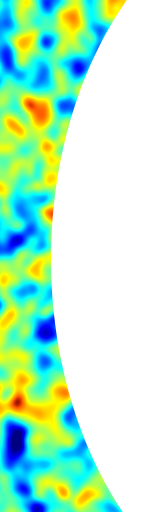
\includegraphics[height=1cm]{sls.png}};
%		\node at (2.5,0) (B) {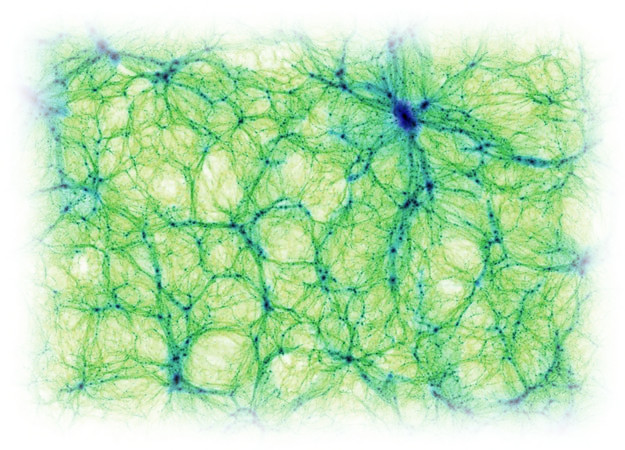
\includegraphics[height=1.5cm]{lss.jpeg}};
%		\node at (5.0,0) (C) {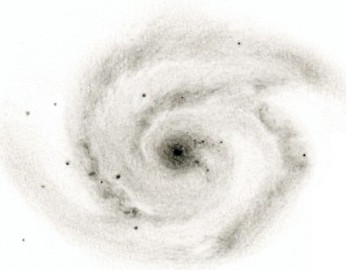
\includegraphics[height=1cm]{galaxy.jpeg}};
%		\node at (7.5,0) (D) {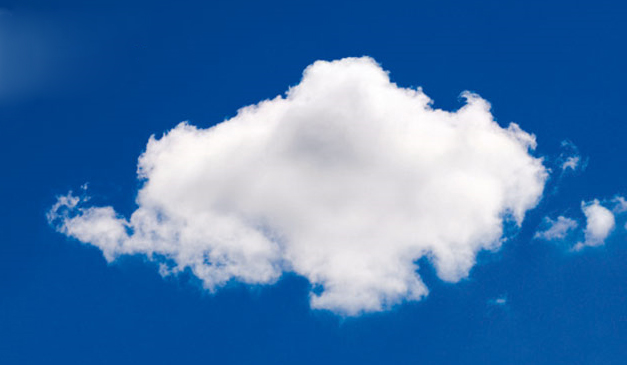
\includegraphics[height=1cm]{cloud.jpg}};
%		\node at (10.0,0) (E) {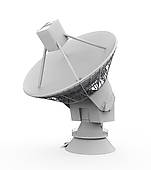
\includegraphics[height=1cm]{telescope.jpg}};
%		\only<1>{\draw [decorate] (0,0) -- (0.5,0);}%
%		\only<2-3>{\draw [decorate] (0,0) -- (2.5,0);}%
%		\only<4-5>{\draw [decorate] (0,0) -- (5.0,0);}%
%		\only<6>{\draw [decorate] (0,0) -- (7.5,0);}%
%		\only<7-10>{\draw [decorate] (0,0) -- (10.0,0);}%
%	\end{tikzpicture}
%	\hspace*{-5mm}\begin{tabular}{ccc}
%		T&E&B\\
%	\only<1>{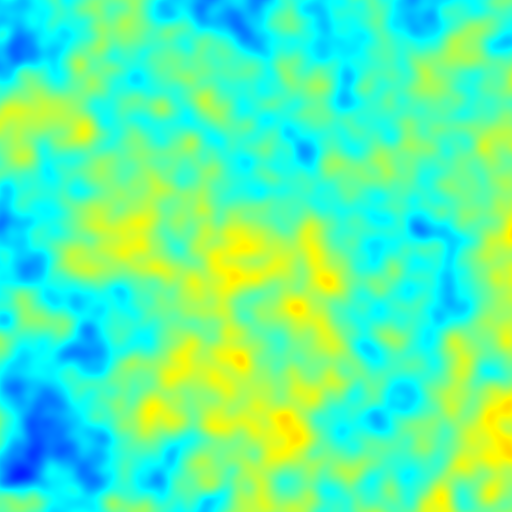
\includegraphics[width=0.35\textwidth]{contaminants/01_cmb_teb_0.png}}%
%	\only<2>{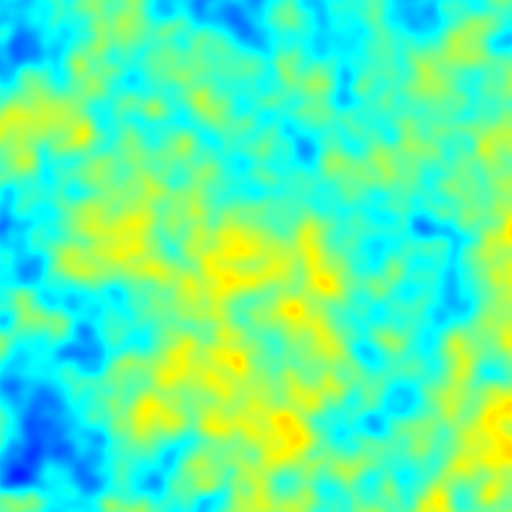
\includegraphics[width=0.35\textwidth]{contaminants/02_lens_teb_0.png}}%
%	\only<3>{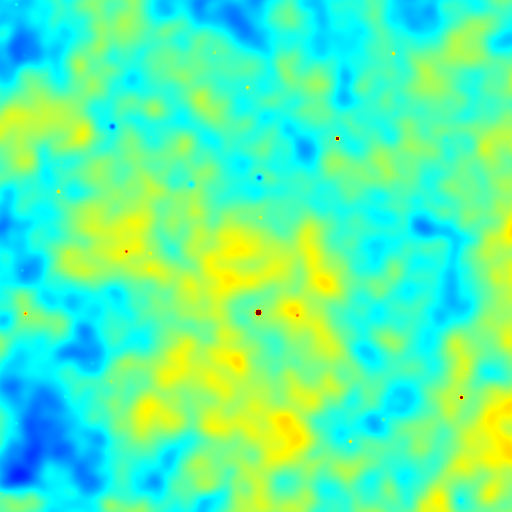
\includegraphics[width=0.35\textwidth]{contaminants/04_sz_teb_0.png}}%
%	\only<4>{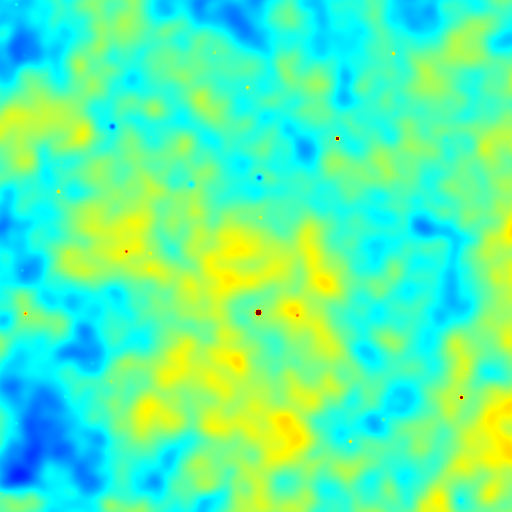
\includegraphics[width=0.35\textwidth]{contaminants/05_faraday_teb_0.png}}%
%	\only<5>{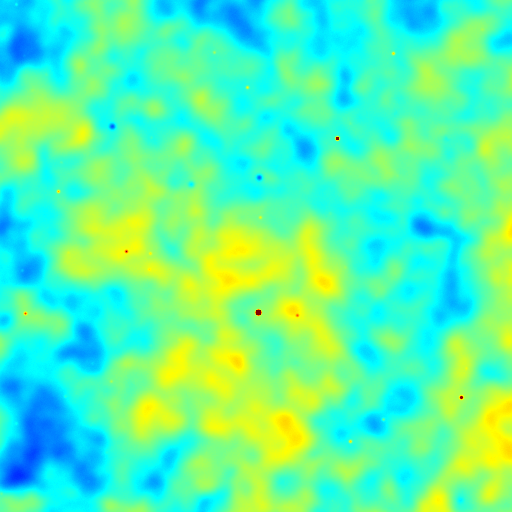
\includegraphics[width=0.35\textwidth]{contaminants/06_dust_teb_0.png}}%
%	\only<6>{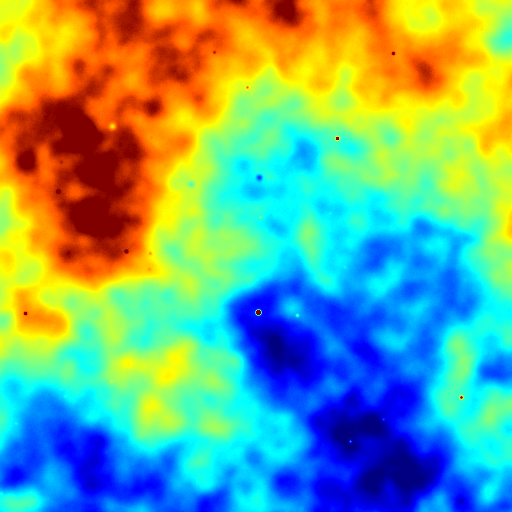
\includegraphics[width=0.35\textwidth]{contaminants/07_atm_teb_0.png}}%
%	\only<7>{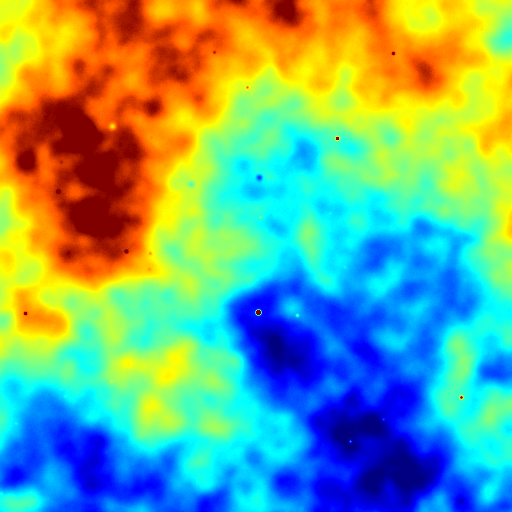
\includegraphics[width=0.35\textwidth]{contaminants/08_polerr_teb_0.png}}%
%	\only<8>{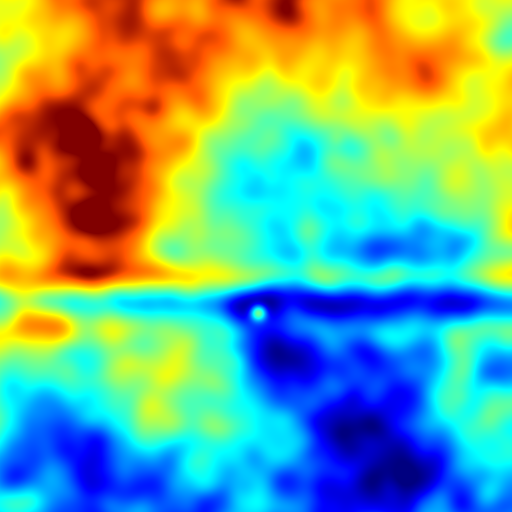
\includegraphics[width=0.35\textwidth]{contaminants/10_beam_teb_0.png}}%
%	\only<9>{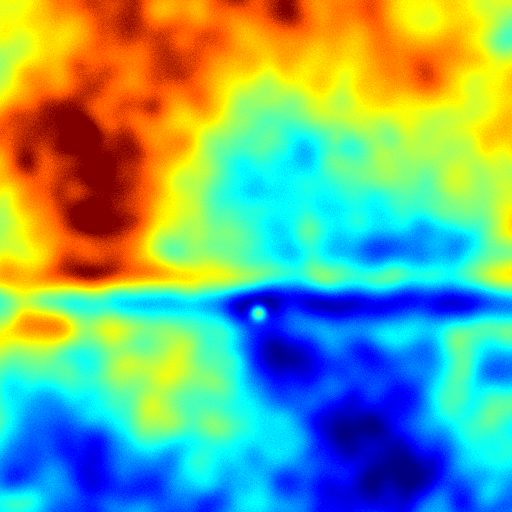
\includegraphics[width=0.35\textwidth]{contaminants/11_noise_teb_0.png}}%
%	\only<10>{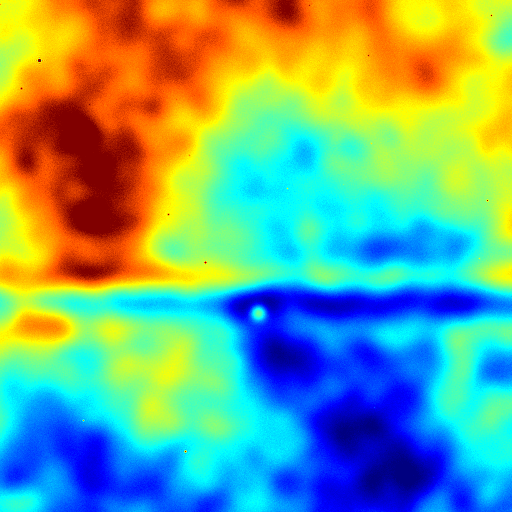
\includegraphics[width=0.35\textwidth]{contaminants/12_glitch_teb_0.png}}%
%	&
%	\only<1>{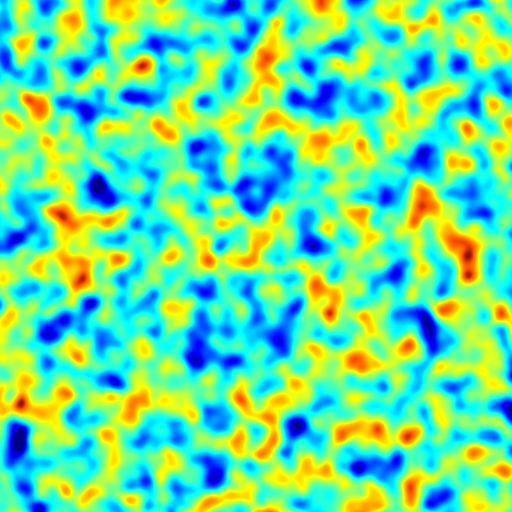
\includegraphics[width=0.35\textwidth]{contaminants/01_cmb_teb_1.png}}%
%	\only<2>{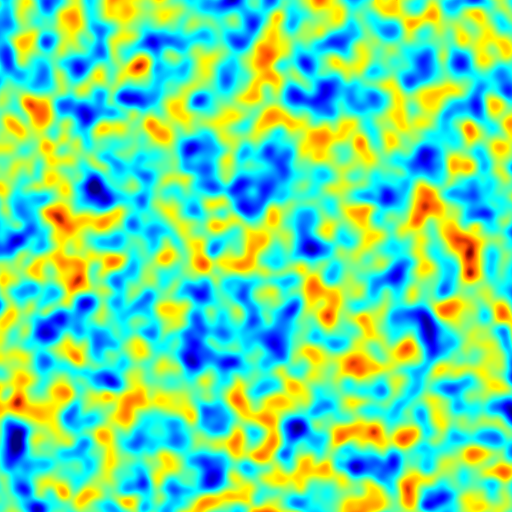
\includegraphics[width=0.35\textwidth]{contaminants/02_lens_teb_1.png}}%
%	\only<3>{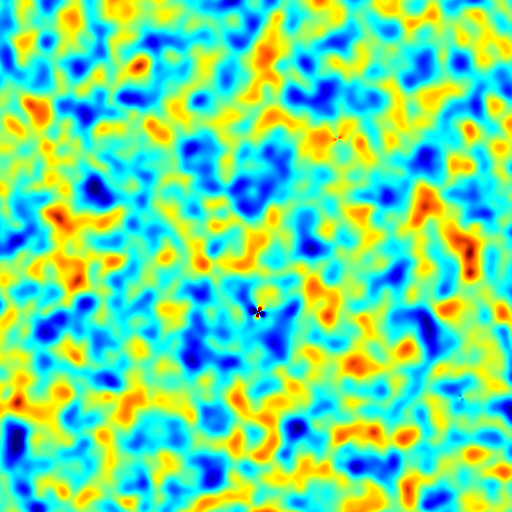
\includegraphics[width=0.35\textwidth]{contaminants/04_sz_teb_1.png}}%
%	\only<4>{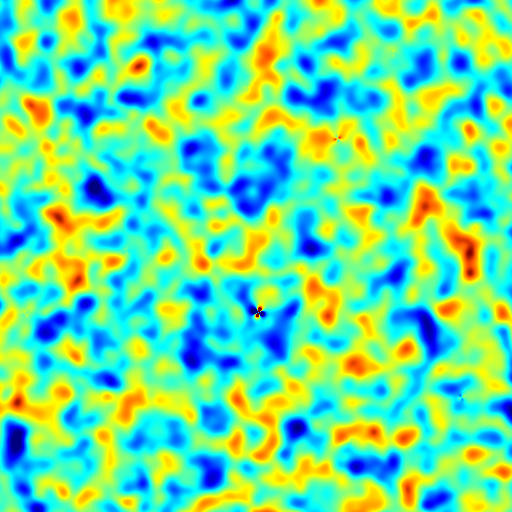
\includegraphics[width=0.35\textwidth]{contaminants/05_faraday_teb_1.png}}%
%	\only<5>{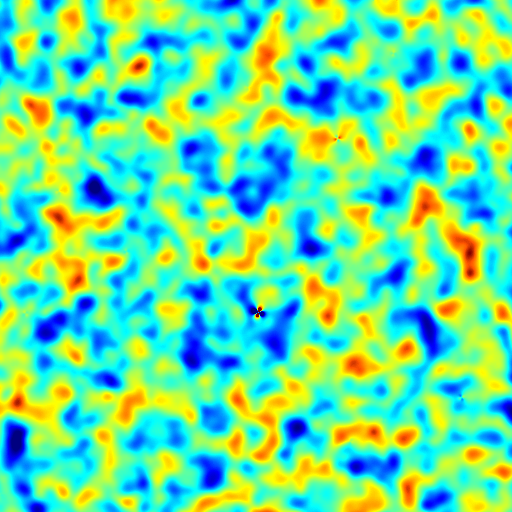
\includegraphics[width=0.35\textwidth]{contaminants/06_dust_teb_1.png}}%
%	\only<6>{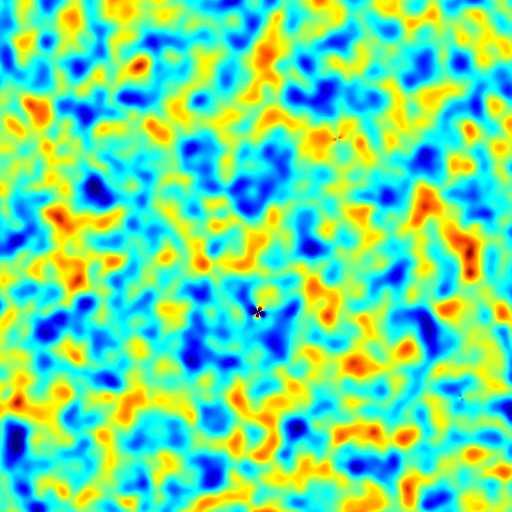
\includegraphics[width=0.35\textwidth]{contaminants/07_atm_teb_1.png}}%
%	\only<7>{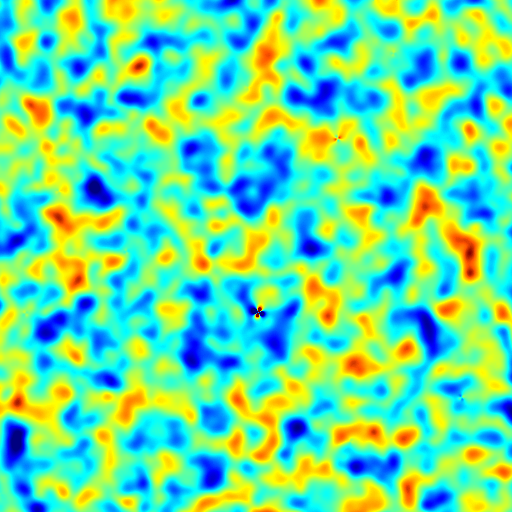
\includegraphics[width=0.35\textwidth]{contaminants/08_polerr_teb_1.png}}%
%	\only<8>{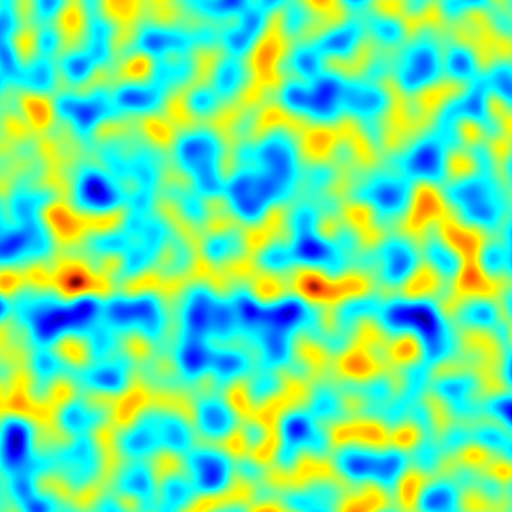
\includegraphics[width=0.35\textwidth]{contaminants/10_beam_teb_1.png}}%
%	\only<9>{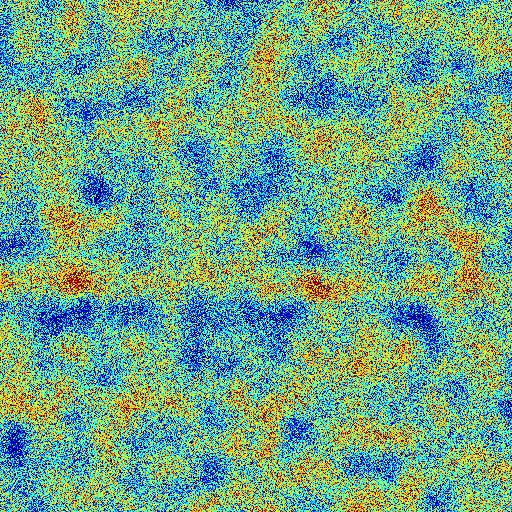
\includegraphics[width=0.35\textwidth]{contaminants/11_noise_teb_1.png}}%
%	\only<10>{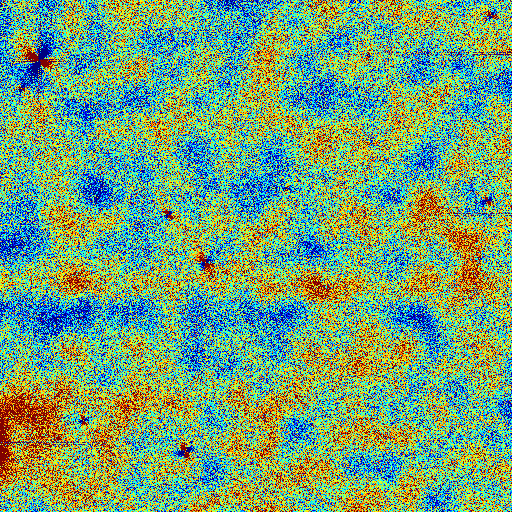
\includegraphics[width=0.35\textwidth]{contaminants/12_glitch_teb_1.png}}%
%	&
%	\only<1>{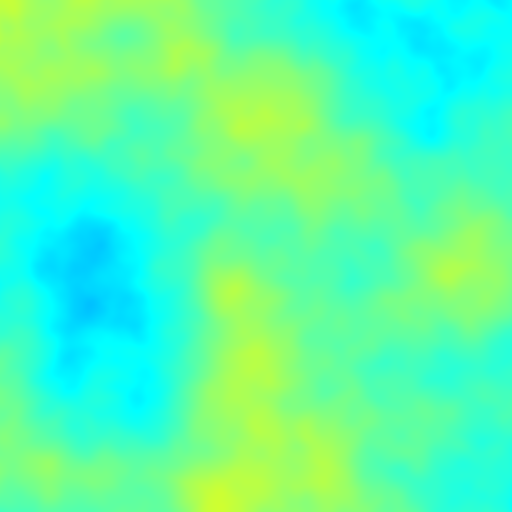
\includegraphics[width=0.35\textwidth]{contaminants/01_cmb_teb_2.png}}%
%	\only<2>{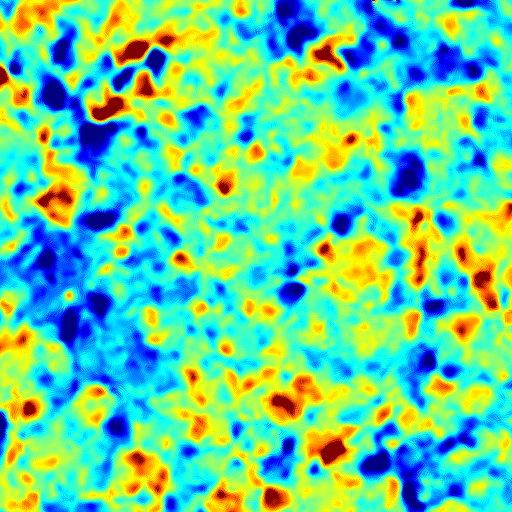
\includegraphics[width=0.35\textwidth]{contaminants/02_lens_teb_2.png}}%
%	\only<3>{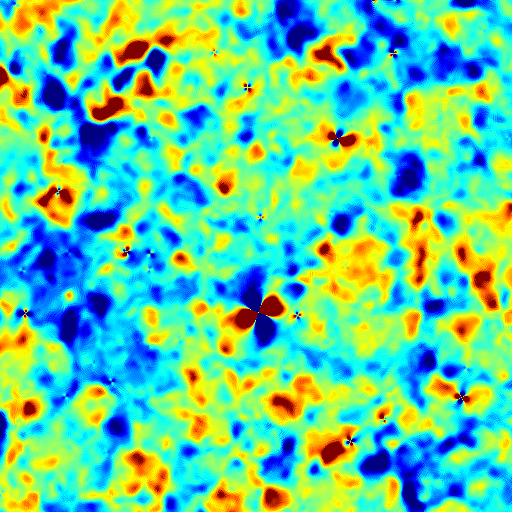
\includegraphics[width=0.35\textwidth]{contaminants/04_sz_teb_2.png}}%
%	\only<4>{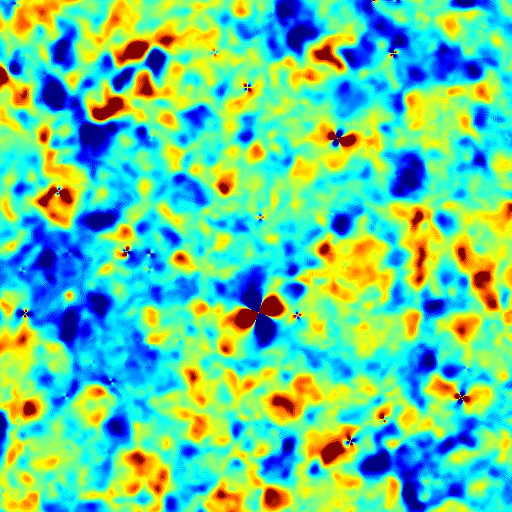
\includegraphics[width=0.35\textwidth]{contaminants/05_faraday_teb_2.png}}%
%	\only<5>{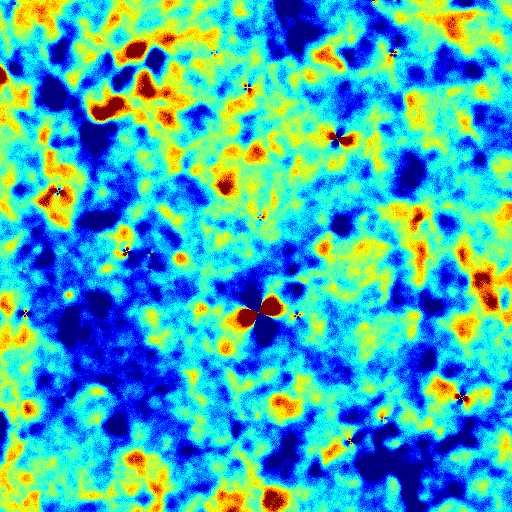
\includegraphics[width=0.35\textwidth]{contaminants/06_dust_teb_2.png}}%
%	\only<6>{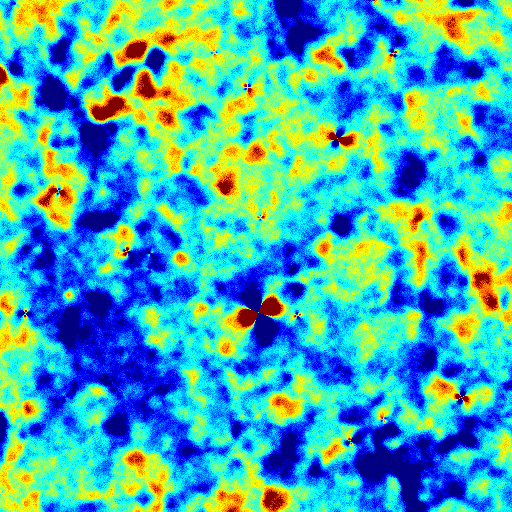
\includegraphics[width=0.35\textwidth]{contaminants/07_atm_teb_2.png}}%
%	\only<7>{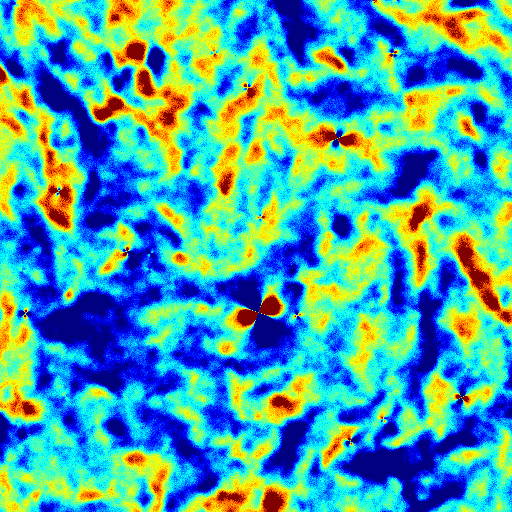
\includegraphics[width=0.35\textwidth]{contaminants/08_polerr_teb_2.png}}%
%	\only<8>{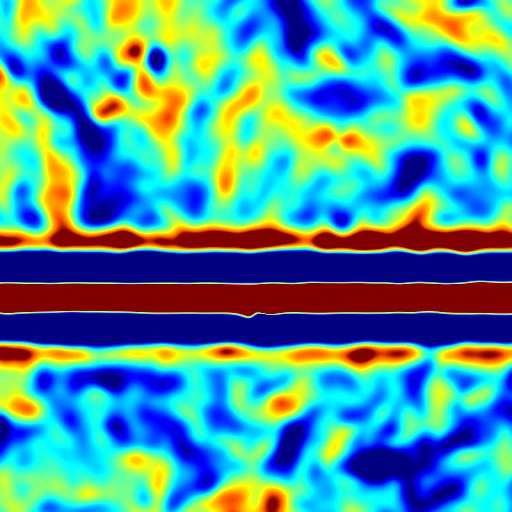
\includegraphics[width=0.35\textwidth]{contaminants/10_beam_teb_2.png}}%
%	\only<9>{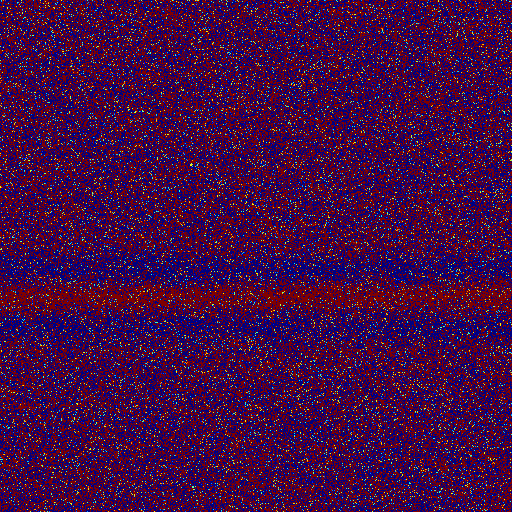
\includegraphics[width=0.35\textwidth]{contaminants/11_noise_teb_2.png}}%
%	\only<10>{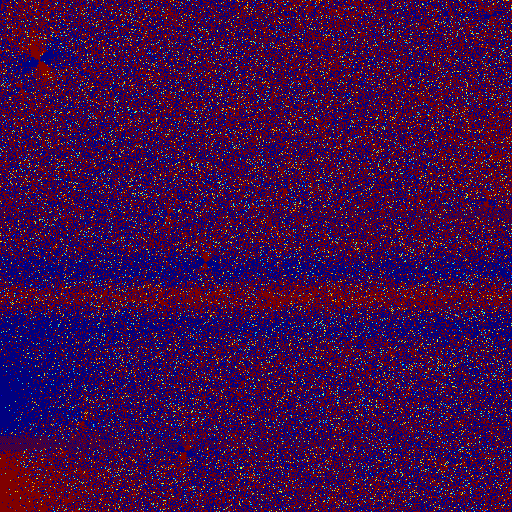
\includegraphics[width=0.35\textwidth]{contaminants/12_glitch_teb_2.png}}%
%	\\
%	{\footnotesize $-500\mu$K\enskip
\includegraphics[width=12mm,height=2mm]{colorbar.png}\enskip$500\mu$K} &
%	{\footnotesize $-20\mu$K\enskip
\includegraphics[width=12mm,height=2mm]{colorbar.png}\enskip$20\mu$K} &
%	{\footnotesize $-1\mu$K\enskip
\includegraphics[width=12mm,height=2mm]{colorbar.png}\enskip$1\mu$K}
%\end{tabular}\hspace*{-5mm}
%\end{frame}
%%    * What telescope measures etc.
%\begin{frame}{What the telescope actually observes}
%	\begin{tikzpicture}[bad/.style={line width=3pt,red}]
%		\node at (0,0) {\begin{tabular}{ccc}
%				T & E & B \\
%				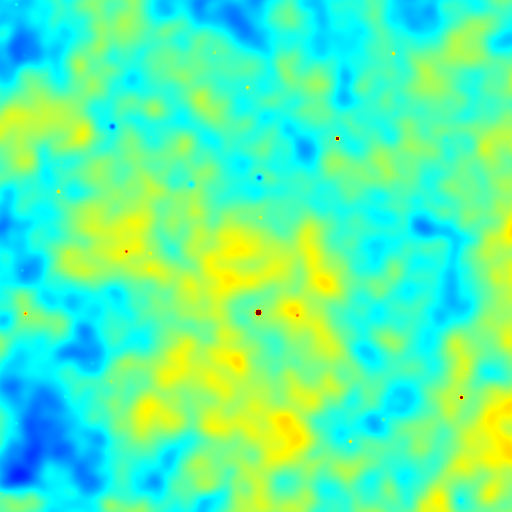
\includegraphics[width=0.30\textwidth]{contaminants/04_sz_teb_0.png} &
%				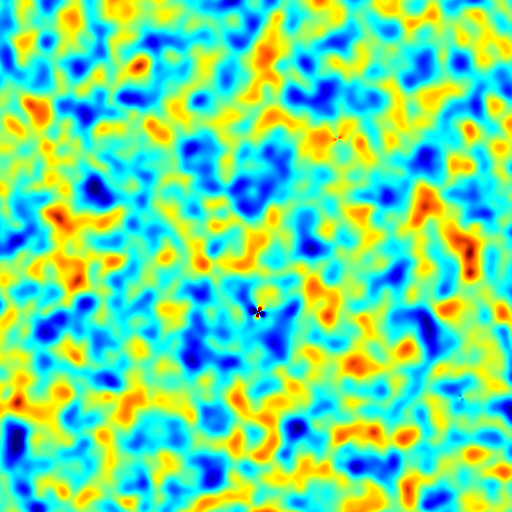
\includegraphics[width=0.30\textwidth]{contaminants/04_sz_teb_1.png} &
%				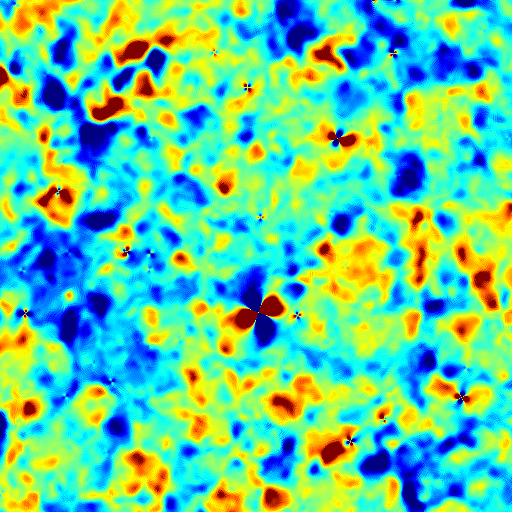
\includegraphics[width=0.30\textwidth]{contaminants/04_sz_teb_2.png}
%		\end{tabular}};
%		\uncover<2->{%
%		\draw[bad] (-5, 1.5) -- (5,-1.8);
%		\draw[bad] (-5,-1.8) -- (5, 1.5);}
%		\node at (0,-4) {\begin{tabular}{ccc}
%				\only<3-4>{T+pol}\only<5->{T} & \uncover<5->{Q} & \uncover<5->{U} \\
%				\only<3-4>{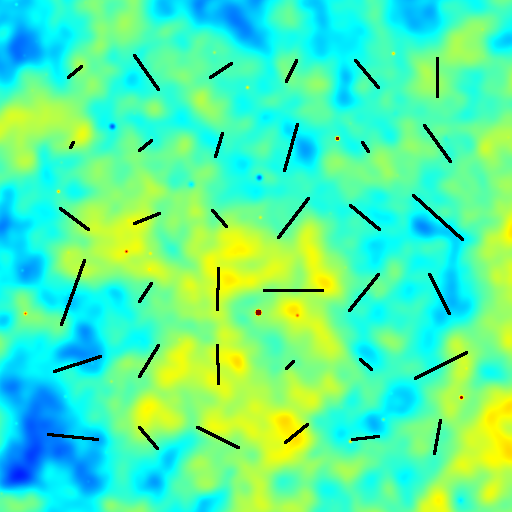
\includegraphics[width=0.30\textwidth]{contaminants/t_polvec.png}}%
%				\only<5->{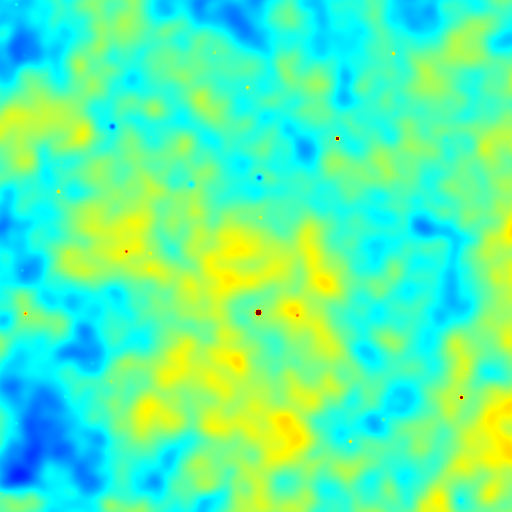
\includegraphics[width=0.30\textwidth]{contaminants/04_sz_tqu_0.png}} &
%				\uncover<5->{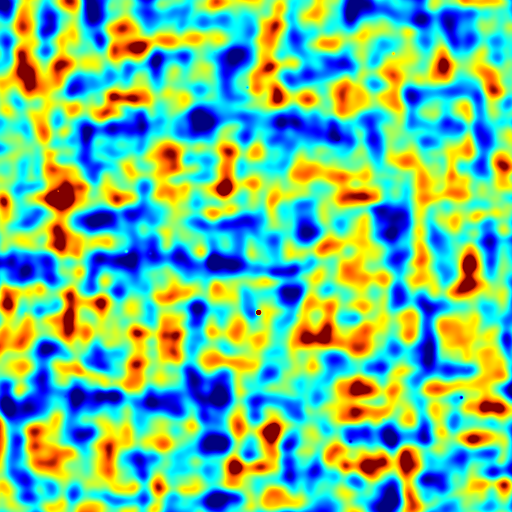
\includegraphics[width=0.30\textwidth]{contaminants/04_sz_tqu_1.png}} &
%				\uncover<5->{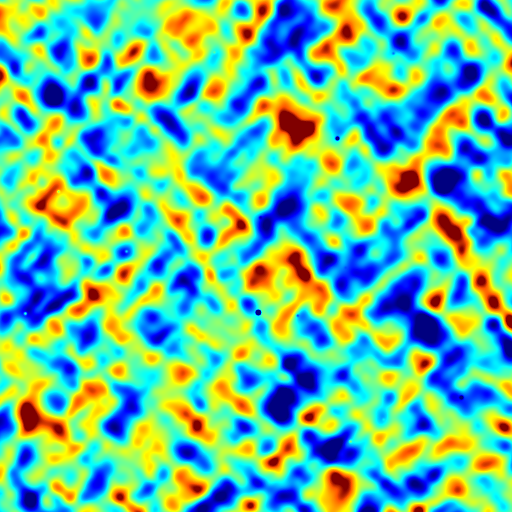
\includegraphics[width=0.30\textwidth]{contaminants/04_sz_tqu_2.png}}
%		\end{tabular}};
%		\uncover<4>{\node at (1.5,-4) {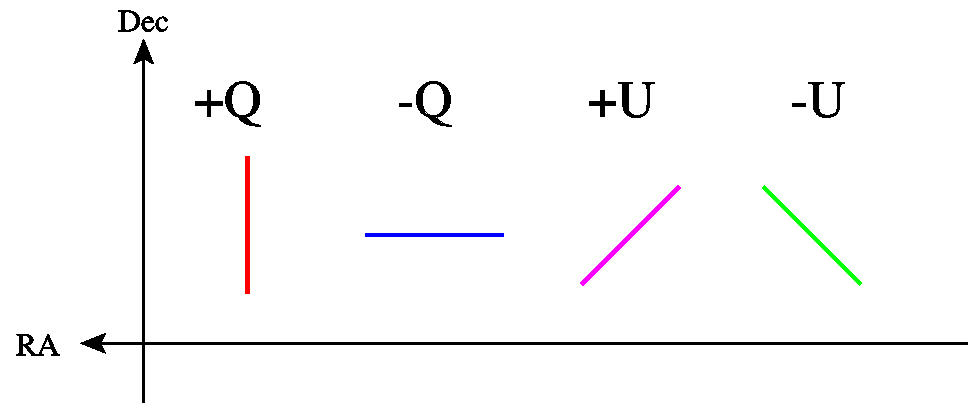
\includegraphics[height=3cm]{qudef_healpix.pdf}};}
%	\end{tikzpicture}
%\end{frame}
%
%\begin{frame}{E,B and Q, U}
%	\begin{center}
%		\only<1>{E and B result from quadrupole-convolutions of Q and U}%
%		\only<2>{Reverse also holds}%
%
%	\scalebox{1.7}{
%		\begin{minipage}{5cm}
%			\begin{align*}
%				\only<1>{%
%				E =& \rmimg{contaminants/queb_0.png}{1cm} \otimes Q + \mimg{contaminants/queb_2.png}{1cm} \otimes U \\
%				B =& \mimg{contaminants/queb_1.png}{1cm} \otimes Q + \rmimg{contaminants/queb_3.png}{1cm} \otimes U}%
%				\only<2>{%
%				Q =& \rmimg{contaminants/ebqu_0.png}{1cm} \otimes E + \mimg{contaminants/ebqu_2.png}{1cm} \otimes B \\
%				U =& \mimg{contaminants/ebqu_1.png}{1cm} \otimes E + \rmimg{contaminants/ebqu_3.png}{1cm} \otimes B}%
%			\end{align*}
%		\end{minipage}}
%	\end{center}
%\end{frame}
%
%\begin{frame}{E, B and Q, U}
%	\begin{center}
%		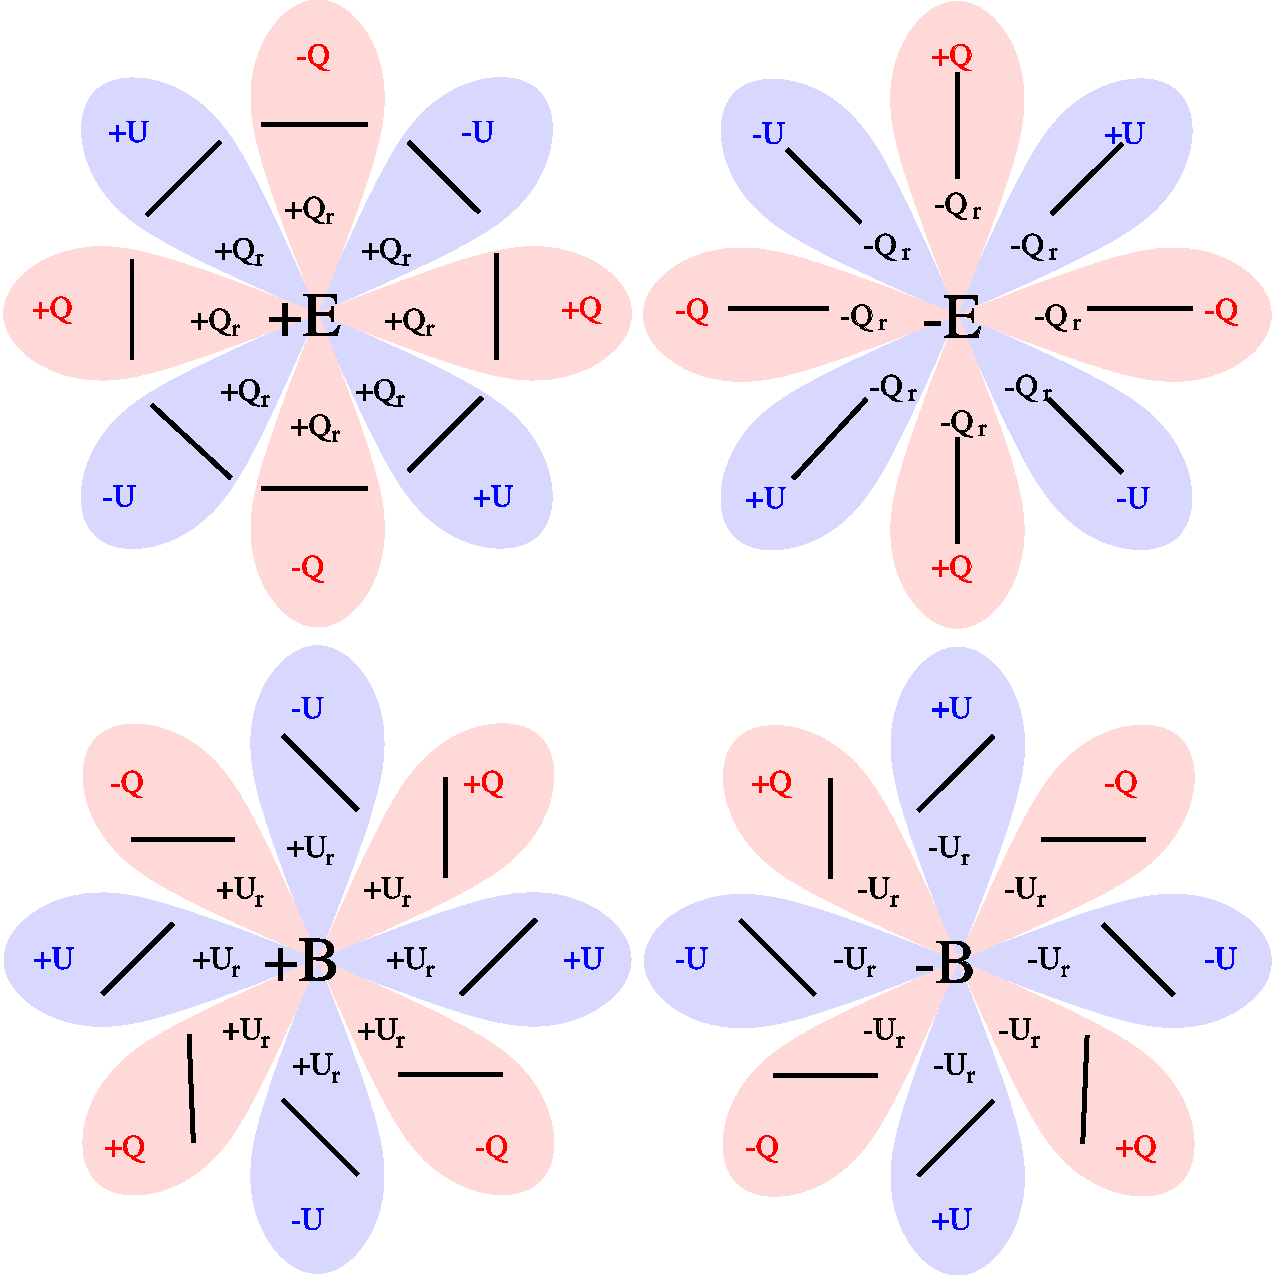
\includegraphics[height=8cm]{EB_healpix.pdf}
%	\end{center}
%\end{frame}
%
%\begin{frame}{Actually only observe linear combinations}
%	\begin{center}
%	\begin{tabular}{c}
%		\only<1>{Detector 1: T+Q}%
%		\only<2>{Detector 2: T+U}%
%		\only<3>{Detector 3: T-Q}%
%		\only<4>{Detector 4: T-U}%
%		\\
%		\only<1>{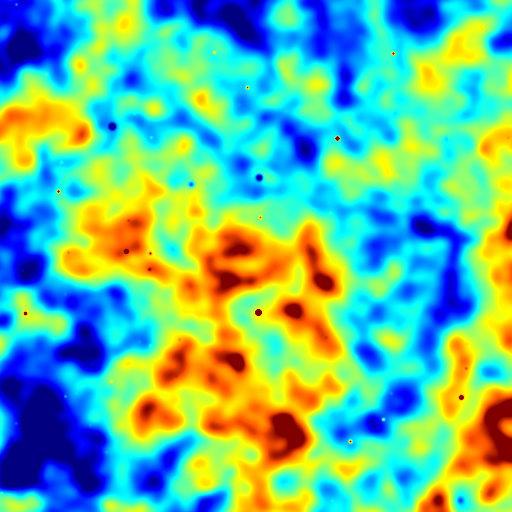
\includegraphics[height=7cm]{contaminants/tqu_lincombs_0.png}}%
%		\only<2>{\includegraphics[height=7cm]{contaminants/tqu_lincombs_1.png}}%
%		\only<3>{\includegraphics[height=7cm]{contaminants/tqu_lincombs_2.png}}%
%		\only<4>{\includegraphics[height=7cm]{contaminants/tqu_lincombs_3.png}}%
%	\end{tabular}
%\end{center}
%\end{frame}
%
%\begin{frame}{Not like a digital camera}
%	\begin{tikzpicture}[bad/.style={line width=8pt,red},scan/.style={thick,red}]
%		\node at (0,0) (A) {\includegraphics[height=3cm]{contaminants/06_dust_teb_0.png}};
%		\uncover<2->{%
%		\node at (1.5,-1) (B) {\includegraphics[height=3cm]{camera.png}};}
%		\uncover<3->{%
%		\draw[bad] (-1.1,-2.1) -- ( 2.6, 1.6);
%		\draw[bad] (-1.1, 1.6) -- ( 2.6,-2.1);}
%		\uncover<4->{%
%		\node at (6,0) (C) {\includegraphics[height=3cm]{contaminants/06_dust_teb_0.png}};}
%		\uncover<5->{%
%		\draw[scan] (5, 1.0) -- (7, 0.9);}
%		\uncover<6->{%
%		\draw[scan] (7, 0.9) -- (5, 0.8);}
%		\uncover<7->{%
%		\draw[scan] (5, 0.8) -- (7, 0.7);}
%		\uncover<8->{%
%		\draw[scan] (7, 0.7) -- (5, 0.6);}
%		\uncover<9->{%
%		\draw[scan] (5, 0.6) -- (7, 0.5);}
%		\uncover<10->{%
%		\draw[scan] (7, 0.5) -- (5, 0.4);}
%		\uncover<11->{%
%		\draw[scan] (5, 0.4) -- (7, 0.3);
%		\draw[scan] (7, 0.3) -- (5, 0.2);
%		\draw[scan] (5, 0.2) -- (7, 0.1);
%		\draw[scan] (7, 0.1) -- (5, 0.0);
%		\draw[scan] (5, 0.0) -- (7,-0.1);
%		\draw[scan] (7,-0.1) -- (5,-0.2);
%		\draw[scan] (5,-0.2) -- (7,-0.3);
%		\draw[scan] (7,-0.3) -- (5,-0.4);
%		\draw[scan] (5,-0.4) -- (7,-0.5);
%		\draw[scan] (7,-0.5) -- (5,-0.6);
%		\draw[scan] (5,-0.6) -- (7,-0.7);
%		\draw[scan] (7,-0.7) -- (5,-0.8);
%		\draw[scan] (5,-0.8) -- (7,-0.9);
%		\draw[scan] (7,-0.9) -- (5,-1.0);
%	\draw[scan] (5,-1.0) -- (7,-1.1);}
%		\uncover<4->{
%		\node at (7.5,-1) (D) {\includegraphics[height=3cm]{telescope2.png}};}
%		\uncover<5->{%
%		\draw[thick,red,->,rounded corners=1mm] (7.5,-2.4) -- (7.5,-2.6) -- (-0.5,-2.6) -- (-0.5,-2.9);
%		\node at (-0.5,-3.00) {\includegraphics[height=0.7mm,width=1.5cm]{contaminants/scanrow100.png}};}
%		\uncover<6->{%
%		\node at ( 1.0,-3.00) {\includegraphics[height=0.7mm,width=1.5cm]{contaminants/scanrow116.png}};}
%		\uncover<7->{%
%		\node at ( 2.5,-3.00) {\includegraphics[height=0.7mm,width=1.5cm]{contaminants/scanrow132.png}};}
%		\uncover<8->{%
%		\node at ( 4.0,-3.00) {\includegraphics[height=0.7mm,width=1.5cm]{contaminants/scanrow148.png}};}
%		\uncover<9->{%
%		\node at ( 5.5,-3.00) {\includegraphics[height=0.7mm,width=1.5cm]{contaminants/scanrow164.png}};}
%		\uncover<10->{%
%		\node at ( 7.0,-3.00) {\includegraphics[height=0.7mm,width=1.5cm]{contaminants/scanrow180.png}};}
%		\uncover<11->{
%		\node at (-0.5,-3.15) {\includegraphics[height=0.7mm,width=1.5cm]{contaminants/scanrow196.png}};
%		\node at ( 1.0,-3.15) {\includegraphics[height=0.7mm,width=1.5cm]{contaminants/scanrow212.png}};
%		\node at ( 2.5,-3.15) {\includegraphics[height=0.7mm,width=1.5cm]{contaminants/scanrow228.png}};
%		\node at ( 4.0,-3.15) {\includegraphics[height=0.7mm,width=1.5cm]{contaminants/scanrow244.png}};
%		\node at ( 5.5,-3.15) {\includegraphics[height=0.7mm,width=1.5cm]{contaminants/scanrow260.png}};
%		\node at ( 7.0,-3.15) {\includegraphics[height=0.7mm,width=1.5cm]{contaminants/scanrow276.png}};
%		\node at (-0.5,-3.30) {\includegraphics[height=0.7mm,width=1.5cm]{contaminants/scanrow292.png}};
%		\node at ( 1.0,-3.30) {\includegraphics[height=0.7mm,width=1.5cm]{contaminants/scanrow308.png}};
%		\node at ( 2.5,-3.30) {\includegraphics[height=0.7mm,width=1.5cm]{contaminants/scanrow324.png}};
%		\node at ( 4.0,-3.30) {\includegraphics[height=0.7mm,width=1.5cm]{contaminants/scanrow340.png}};
%		\node at ( 5.5,-3.30) {\includegraphics[height=0.7mm,width=1.5cm]{contaminants/scanrow356.png}};
%		\node at ( 7.0,-3.30) {\includegraphics[height=0.7mm,width=1.5cm]{contaminants/scanrow372.png}};
%		\node at (-0.5,-3.45) {\includegraphics[height=0.7mm,width=1.5cm]{contaminants/scanrow388.png}};}
%	\end{tikzpicture}
%	\begin{center}
%		\uncover<12->{\large Time-ordered data (TOD)}
%	\end{center}
%\end{frame}
%%    * TOD
%\begin{frame}{Example TOD}
%	\begin{center}
%		\vspace{-1.5cm}
%		\begin{tikzpicture}
%			\node at (0,0) {\includegraphics[width=\textwidth]{example_tod.png}};
%			\uncover<7->{%
%			\draw (-1.2, 0.4) ellipse (4mm and 7mm);
%			\draw (2.70,0.7) ellipse (4mm and 12mm);}
%		\end{tikzpicture}
%		\uncover<2->{%
%		\begin{block}{Ingredients}
%			\begin{columns}
%				\begin{column}{5cm}
%					\begin{itemize}
%						\item<2-> 90\% atmospheric noise
%						\item<3-> 10\% instrumental noise
%						\item<4-> 0.4\% T-modes
%					\end{itemize}
%				\end{column}
%				\begin{column}{5cm}
%					\begin{itemize}
%						\item<5-> 0.002\% E-modes
%						\item<6-> 0.0002\% B-modes
%						\item<7-> and a few glitches
%					\end{itemize}
%				\end{column}
%			\end{columns}
%		\end{block}}
%	\end{center}
%\end{frame}
%%    * Image reconstruction
%\begin{frame}{Recovering the sky}
%	Can model TOD as linear combination of CMB and noise:
%	\[ d = {\color{green}P}{\color{blue}s} + {\color{red}n} \]
%	with TOD $d$,
%	scan pattern + telescope response {\color{green} $P$},
%	cmb map {\color{blue} $s$}, gaussian noise {\color{red} $n$} with cov {\color{red}$N$}.
%	Then
%	\[ {\color{blue}s} = ({\color{green}P}^T{\color{red}N}^{-1}{\color{green}P})^{-1}{\color{green}P}^T{\color{red}N}^{-1}d \]
%	is an optimal estimator.
%\end{frame}
%%    * Beat down noise (white)
%\begin{frame}{Throw samples at it to beat down noise}
%	\begin{center}
%	\hspace*{-1.4cm}\begin{tabular}{ccc}
%		T & Q & U \\
%		\only<1>{%
%		\includegraphics[height=4cm]{maps/scansims/scansims_000_0.png} &
%		\includegraphics[height=4cm]{maps/scansims/scansims_000_1.png} &
%		\includegraphics[height=4cm]{maps/scansims/scansims_000_2.png}}%
%		\only<2>{%
%		\includegraphics[height=4cm]{maps/scansims/scansims_001_0.png} &
%		\includegraphics[height=4cm]{maps/scansims/scansims_001_1.png} &
%		\includegraphics[height=4cm]{maps/scansims/scansims_001_2.png}}%
%		\only<3>{%
%		\includegraphics[height=4cm]{maps/scansims/scansims_002_0.png} &
%		\includegraphics[height=4cm]{maps/scansims/scansims_002_1.png} &
%		\includegraphics[height=4cm]{maps/scansims/scansims_002_2.png}}%
%		\only<4>{%
%		\includegraphics[height=4cm]{maps/scansims/scansims_003_0.png} &
%		\includegraphics[height=4cm]{maps/scansims/scansims_003_1.png} &
%		\includegraphics[height=4cm]{maps/scansims/scansims_003_2.png}}%
%		\only<5>{%
%		\includegraphics[height=4cm]{maps/scansims/scansims_004_0.png} &
%		\includegraphics[height=4cm]{maps/scansims/scansims_004_1.png} &
%		\includegraphics[height=4cm]{maps/scansims/scansims_004_2.png}}%
%		\only<6>{%
%		\includegraphics[height=4cm]{maps/scansims/scansims_005_0.png} &
%		\includegraphics[height=4cm]{maps/scansims/scansims_005_1.png} &
%		\includegraphics[height=4cm]{maps/scansims/scansims_005_2.png}}%
%		\only<7>{%
%		\includegraphics[height=4cm]{maps/scansims/scansims_006_0.png} &
%		\includegraphics[height=4cm]{maps/scansims/scansims_006_1.png} &
%		\includegraphics[height=4cm]{maps/scansims/scansims_006_2.png}}%
%		\only<8>{%
%		\includegraphics[height=4cm]{maps/scansims/scansims_007_0.png} &
%		\includegraphics[height=4cm]{maps/scansims/scansims_007_1.png} &
%		\includegraphics[height=4cm]{maps/scansims/scansims_007_2.png}}%
%		\only<9>{%
%		\includegraphics[height=4cm]{maps/scansims/scansims_008_0.png} &
%		\includegraphics[height=4cm]{maps/scansims/scansims_008_1.png} &
%		\includegraphics[height=4cm]{maps/scansims/scansims_008_2.png}}%
%		\only<10>{%
%		\includegraphics[height=4cm]{maps/scansims/scansims_009_0.png} &
%		\includegraphics[height=4cm]{maps/scansims/scansims_009_1.png} &
%		\includegraphics[height=4cm]{maps/scansims/scansims_009_2.png}}%
%		\only<11>{%
%		\includegraphics[height=4cm]{maps/scansims/scansims_010_0.png} &
%		\includegraphics[height=4cm]{maps/scansims/scansims_010_1.png} &
%		\includegraphics[height=4cm]{maps/scansims/scansims_010_2.png}}%
%		\only<12>{%
%		\includegraphics[height=4cm]{maps/scansims/scansims_011_0.png} &
%		\includegraphics[height=4cm]{maps/scansims/scansims_011_1.png} &
%		\includegraphics[height=4cm]{maps/scansims/scansims_011_2.png}}%
%		\only<13>{%
%		\includegraphics[height=4cm]{maps/scansims/scansims_012_0.png} &
%		\includegraphics[height=4cm]{maps/scansims/scansims_012_1.png} &
%		\includegraphics[height=4cm]{maps/scansims/scansims_012_2.png}}%
%		\only<14>{%
%		\includegraphics[height=4cm]{maps/scansims/scansims_013_0.png} &
%		\includegraphics[height=4cm]{maps/scansims/scansims_013_1.png} &
%		\includegraphics[height=4cm]{maps/scansims/scansims_013_2.png}}%
%		\only<15>{%
%		\includegraphics[height=4cm]{maps/scansims/scansims_014_0.png} &
%		\includegraphics[height=4cm]{maps/scansims/scansims_014_1.png} &
%		\includegraphics[height=4cm]{maps/scansims/scansims_014_2.png}}%
%		\only<16>{%
%		\includegraphics[height=4cm]{maps/scansims/scansims_015_0.png} &
%		\includegraphics[height=4cm]{maps/scansims/scansims_015_1.png} &
%		\includegraphics[height=4cm]{maps/scansims/scansims_015_2.png}}%
%		\only<17>{%
%		\includegraphics[height=4cm]{maps/scansims/scansims_016_0.png} &
%		\includegraphics[height=4cm]{maps/scansims/scansims_016_1.png} &
%		\includegraphics[height=4cm]{maps/scansims/scansims_016_2.png}}%
%		\only<18>{%
%		\includegraphics[height=4cm]{maps/scansims/scansims_017_0.png} &
%		\includegraphics[height=4cm]{maps/scansims/scansims_017_1.png} &
%		\includegraphics[height=4cm]{maps/scansims/scansims_017_2.png}}%
%	\end{tabular}\hspace*{-1.4cm}
%\end{center}
%\end{frame}
%%    * Beat down noise (full)
%\begin{frame}{What real noise looks like}
%	\begin{center}
%	\only<1>{\hspace*{-1cm}\includegraphics[height=8cm]{maps/scanreal/map00_small_0_crop.png}}%
%	\only<2>{\hspace*{-1cm}\includegraphics[height=8cm]{maps/scanreal/map01_small_0_crop.png}}%
%	\only<3>{\hspace*{-1cm}\includegraphics[height=8cm]{maps/scanreal/map02_small_0_crop.png}}%
%	\only<4>{\hspace*{-1cm}\includegraphics[height=8cm]{maps/scanreal/map03_small_0_crop.png}}%
%	\only<5>{\hspace*{-1cm}\includegraphics[height=8cm]{maps/scanreal/map04_small_0_crop.png}}%
%	\only<6>{\hspace*{-1cm}\includegraphics[height=8cm]{maps/scanreal/map05_small_0_crop.png}}%
%	\only<7>{\hspace*{-1cm}\includegraphics[height=8cm]{maps/scanreal/map06_small_0_crop.png}}%
%	\only<8>{\hspace*{-1cm}\includegraphics[height=8cm]{maps/scanreal/map07_small_0_crop.png}}%
%	\only<9>{\hspace*{-1cm}\includegraphics[height=8cm]{maps/scanreal/map08_small_0_crop.png}}%
%	\only<10>{\hspace*{-1cm}\includegraphics[height=8cm]{maps/scanreal/map09_small_0_crop.png}}%
%	\only<11>{\hspace*{-1cm}\includegraphics[height=8cm]{maps/scanreal/map10_small_0_crop.png}}%
%	\end{center}
%\end{frame}
%% 20 * List of instruments trying to do this
%%    * ACT
%\begin{frame}{ACT site PWV}
%	\centering
%	\includegraphics[width=\textwidth]{pwv_chajnantor_eso.jpeg}
%\end{frame}
%% 22 * Example CMB image from 2014 ACTPol article - before and after bandpass
%%    * Planck comparison?
%%    * Resulting image is not pristine CMB due to noise and systematic effects.
%%      Lensing, SZ, point sources, CIB, unresolved AGNs, diffuse galactic emission
%%    * But that's fine!
%%      Systematic effects as S/N increases: ignorable -> nuisance -> problem -> signal
%%    * Split image into CMB + rest, highlight ACT goals
%\begin{frame}
%	\centering
%	\begin{tabular}{c}
%		\only<1>{Total signal}%
%		\only<2>{CMB (Wiener)}%
%		\only<3>{Remainder}%
%		\only<4>{Total signal}%
%		\\
%		\only<1>{\includegraphics[width=0.7\textwidth]{maps/crop/coadd.png}}%
%		\only<2>{\includegraphics[width=0.7\textwidth]{maps/crop/cmb.png}}%
%		\only<3>{\includegraphics[width=0.7\textwidth]{maps/crop/nocmb.png}}%
%		\only<4>{\includegraphics[width=0.7\textwidth]{maps/crop/coadd.png}}%
%		\\
%		$\pm 250 \mu$K, $4.26^\circ \times 4.26^\circ$
%	\end{tabular}
%\end{frame}
%% 25 * ACT goals: CMB lensing (w B-modes), High-l CMB, SZ, (low-l B-modes), (ptsrcs)
%%    * Lensing
%%      - Illustration of effect
%\begin{frame}{Lensing distorts the CMB}
%	\begin{center}
%		\begin{tikzpicture}
%			\only<1>{\node at (0,0) {\includegraphics[height=7cm]{lensing/T.png}};}%
%			\only<2>{\node at (0,0) {\includegraphics[height=7cm]{lensing/T.png}};}%
%			\only<3>{\node at (0,0) {\includegraphics[height=7cm]{lensing/TlT.png}};}%
%			\only<4-5>{\node at (0,0) {\includegraphics[height=7cm]{lensing/TsT.png}};}%
%			\only<2-4>{\node at (0,0) {\includegraphics[height=7cm]{lensing/phi_contours.png}};}%
%		\end{tikzpicture}
%
%		\only<1>{Unlensed\uncover<0>{p}}%
%		\only<2>{Gravitational potential}%
%		\only<3>{Lensed\uncover<0>{p}}%
%		\only<4>{Lensed x10\uncover<0>{p}}%
%		\only<5>{Non-Gaussian\uncover<0>{p}}%
%	\end{center}
%\end{frame}
%
%\begin{frame}{Lensing distorts the CMB Polarization}
%	\begin{center}
%		\hspace*{-3mm}
%		\begin{tabular}{cc}
%			{\bf Q} ($\pm 20\mu$K) & {\bf U} ($\pm 20\mu$K) \\
%			\only<1>{\includegraphics[height=5.5cm]{lensing/EBQ.png}}%
%			\only<2>{\includegraphics[height=5.5cm]{lensing/EBlQ.png}}%
%			&
%			\only<1>{\includegraphics[height=5.5cm]{lensing/EBU.png}}%
%			\only<2>{\includegraphics[height=5.5cm]{lensing/EBlU.png}}%
%		\end{tabular}
%
%		\only<1>{Unlensed}%
%		\only<2>{Lensed}%
%	\end{center}
%\end{frame}
%
%\begin{frame}{Lensing distorts E and B}
%	\begin{center}
%		\hspace*{-3mm}
%		\begin{tabular}{cc}
%			{\bf E} ($\pm 20\mu$K) & {\bf B} ($\pm 0.5\mu$K) \\
%			\only<1>{\includegraphics[height=5.5cm]{lensing/E.png}}%
%			\only<2>{\includegraphics[height=5.5cm]{lensing/EBlE.png}}%
%			&
%			\only<1>{\includegraphics[height=5.5cm]{lensing/B.png}}%
%			\only<2>{\includegraphics[height=5.5cm]{lensing/EBlB.png}}%
%		\end{tabular}
%
%		\only<1>{Unlensed}%
%		\only<2>{Lensed}%
%	\end{center}
%\end{frame}
%      - What it helps with ((geometric degeneracy), neutrino mass, bias, dark energy(how?))
%      - ACT results
%      - Planck dominates
% 30 * High-l CMB
\begin{frame}{ACTPol first-season polarization maps}
	\centering
	\begin{tabular}{m{2mm}m{10cm}}
		\rotatebox{90}{sum map} & \includegraphics[width=\textwidth]{actpol_2014_TQUEB.pdf} \\
		\rotatebox{90}{diff map}& \includegraphics[width=\textwidth]{actpol_2014_noise_TEB.pdf}
	\end{tabular}
\end{frame}
\begin{frame}{ACT angular power spectra}
	\centering
	\includegraphics[width=\textwidth]{tteepaper.pdf}
\end{frame}
%      - What it helps with
%      - ACT results
%      - With others
% 35 * SZ
%      - tSZ, kSZ

\begin{frame}{Sunyaev Zel'dovich effect}
	\centering
	\begin{tikzpicture}
		\node at (0,0) {\includegraphics[height=6cm]{sz_illustration_van_speybroeck.png}};
		\uncover<2>{\node at (5.5,0) {\includegraphics[height=5cm]{sz_intensity_carlstrom.jpeg}};}
		\uncover<3-4>{\node at (5.5,-0.3) {\includegraphics[height=4.5cm]{sz_temperature.jpeg}};}
		\node at (0,-3.2) {\footnotesize{Credit: Van Speybroeck}};
		\uncover<2-4>{\node at (5.5,-3.1) {\footnotesize{Credit: Carlstrom}};};
		\uncover<4->{
			\node at (2.8,-4.0) {
				\includegraphics[height=1cm]{maps/sz1.png}
				\includegraphics[height=1cm]{maps/sz2.png}
				\includegraphics[height=1cm]{maps/sz3.png}
				\includegraphics[height=1cm]{maps/sz4.png}
				\includegraphics[height=1cm]{maps/sz5.png}
				\includegraphics[height=1cm]{maps/sz6.png}
				\includegraphics[height=1cm]{maps/sz7.png}
				\includegraphics[height=1cm]{maps/sz8.png}
				\includegraphics[height=1cm]{maps/sz9.png}
			};
			\node at (2.8,-4.6) {\footnotesize{Credit: Planck}};
		}
		\uncover<5>{
			\node[text width=5cm] at (5.5,0) {
				\begin{itemize}
					\item Distance independent: Detect massive clusters at any distance!
					\item Given pressure profile model: Measure mass and physical size of cluster
					\item Probe cluster mass distribution as function of redshift
				\end{itemize}
			};
		}
	\end{tikzpicture}
\end{frame}
\begin{frame}{ACT Measurements}
	\includegraphics[width=\textwidth]{act_sz_clusters.eps} \\
	\begin{tikzpicture}
		\node[text width=5cm] at (0,0.5) {
			\begin{itemize}
				\item ACT detected 68 clusters
				\item Cosmology limited by pressure profile
				\item ACTPol analysis ongoing
			\end{itemize}
		};
		\node at (5,0) {\includegraphics[width=4cm]{act_sz_cosmology.eps}};

	\end{tikzpicture}

\end{frame}

\begin{frame}{Kinematic SZ}
	\begin{tikzpicture}
		\node at (0,0) {\includegraphics[height=6cm]{sz_illustration_van_speybroeck.png}};
		\node at (5.5,-0.3) {\includegraphics[height=4.5cm]{sz_temperature.jpeg}};
		\node at (0,-3.2) {\footnotesize{Credit: Van Speybroeck}};
		\node at (5.5,-3.1) {\footnotesize{Credit: Carlstrom}};
		\uncover<2->{
		\draw [thick,red,->] (-1.7,-0.0) -- +(0,-0.5);
		\draw [thick,red,->] (-1.3,-0.35) -- +(0,-0.5);
		\draw [thick,red,->] (-0.9,-0.45) -- +(0,-0.5);
		\draw [thick,red,->] (-0.5,-0.50) -- +(0,-0.5);
		\draw [thick,red,->] ( 0.5,-0.40) -- +(0,-0.5);
		\draw [thick,red,->] ( 0.9,-0.30) -- +(0,-0.5);
		\draw [thick,red,->] ( 1.3, 0.30) -- +(0,-0.5);}
		\uncover<3->{
			\draw [thick,red] (3.94,1.089) -- +(0.25,0.0) -- +(0.50,0.01) -- +(0.75,0.022) -- +(1.00,0.035) -- +(1.5,0.067)-- +(2.0,0.090) -- +(2.5,0.098) -- +(3.88,0.110);
		}
	\end{tikzpicture}
\end{frame}

\begin{frame}{Kinematic SZ}
	\begin{tikzpicture}
		\node at (0,0) {\includegraphics[height=8cm]{sz_act_boss_sudeep.jpeg}};
		\node at (5.5,-2) {\includegraphics[width=6cm]{actpol_ksz_detection.png}};
		\node[text width=7cm] at (5.5,2) {
			\begin{itemize}
				\item Very faint ($\sim 20$ times weaker than kSZ)
				\item Hard to distinguish from CMB + tSZ
				\item First detection by ACT in 2012 via pairwise comparison of 5000 galaxies

			\end{itemize}
		};
	\end{tikzpicture}
\end{frame}
%      - first detection of kSZ?
% 40 * Summary of ACT firsts
%    * Future: Full ACTPol and Advanced act
\begin{frame}
	\centering
	\hspace*{-0.8cm}\includegraphics[width=12.5cm]{advact_sky_coverage.png} \\
	\includegraphics[width=\textwidth]{advact_multichroic.png}
\end{frame}
\begin{frame}
	\centering
	\hspace*{-1cm}\begin{tikzpicture}
		\node at (0, 2) {\includegraphics[height=5.2cm]{advact_polspec_forecast.png}};
		\node at (0.3,-2.1) {\includegraphics[height=3cm,width=5cm]{advact_lensing_forecast_blake.png}};
		\node at (0.5, -1) {\small CMB lensing};
		\node[red] at (0.3,-2.5) {$\sim220\sigma$};
		\node at (0.3,-3.2) {\footnotesize{Credit: Blake Sherwin}};
		\node at (5, 2) {\includegraphics[width=4.3cm]{advact_cluster_forecast.pdf}};
		\node at (5,-2.05) {\includegraphics[width=4cm]{advact_dsfg_forecast.pdf}};
	\end{tikzpicture}
\end{frame}
% 45 * End

% Pretty long!





% ACT main science stuff
%  Power spectra
%  * High-l TT -> ns(?), Neff
%  * High-l EE -> as TT but less foregrounds (CIB, agn)
%  CMB lensing
%  * Mid-high l TT, EE -> lensing
%  * Mid-l  BB -> lensing B-modes. No cosmic variance from non-lensing
%  Individual sources
%  * SZ clusters -> tSZ, kSZ. kSZ better but only detectable in aggregate to us
%  * Point source catalogue -> lots of high-redshift stuff (but how much of it is new?)
%  (Stacked sources)

% Overall thread
%  * Will talk about recent act CMB measurements
%  * CMB is blah blah, nice because blah blah, monopole, dipole, etc.
%  * Physics in the CMB, T, E and B
%  * What happens to the CMB on its way to us, good+bad
%  * How you go about trying to measure it (scanning etc)
%  * Short history of observations
%    - map with early experiments and early results
%      * Monopole: Penzias, Wilson 1964
%      * Dipole:   Henry 1971
%      * Blackbody: COBE FIRAS 1992
%      * Quadrupole to l\sim 15: COBE DMR 1992
%      * WMAP + others
%    - map with some current experiments
%      * Planck, BICEP+CLASS+SPIDER (prim B), ACT+SPT (high-l)
%  * ACT and ACTPol, 5000 m in Atacama, Chile, observed from, pol from, high resolution (for CMB)





% 45 min talk, should have time to go through how we make maps
% Reuse foreground lensing too?
%
% === Map stuff ===
% Full-sky planck cmb
% zoom on patch
% compare with actpol, looks similar due to large-mode dominance
% gradually subtract large-scale modes to reveal all the small-scale modes
% highlight non-cmb features: point sources, clusters
% illustrate white noise vs correlated noise
% actpol TOD power spectrum -> actpol noise angular power spectrum
% map distortions - flat sky, boosting, lensing
%
% === Telescopes ===
% Planck: Full-sky, multi-frequency, shallow, low-res (l<2500)
% Bicep:  Small patch, very deep, low-res
% Polarbear: Small patch, deep, ?-res
% ACT,SPT: Small-medium patches, deep, high-res (l<10000)

% === Physics ===
% What can you do with high resolution?
%  ns, Neff
%  lensing -> neutrino mass, modified gravity tests?, measure galaxy bias by cross-correlation
%   explain why high res is good for lensing
%   in the low noise limit you need more modes to beat down cosmic variance
%  sz clusters -> Tsz, Ksz. Ksz probes velocity field
%  point sources - are these useful?

% === ACTPol status and plans ===
% Analysing S2 of actpol data, preparing for S3 observing with new frequencies
% Advanced actpol

\begin{frame}
	\centering
	\begin{tabular}{c}
		\only<1>{Planck}%
		\only<2>{Planck+actpol}%
		\only<3>{Planck+actpol $\ell>2000$}%
		\only<4>{Planck $\ell>2000$}%
		\\
		\only<1>{\includegraphics[width=0.7\textwidth]{maps/crop/planck.png}}%
		\only<2>{\includegraphics[width=0.7\textwidth]{maps/crop/coadd.png}}%
		\only<3>{\includegraphics[width=0.7\textwidth]{maps/crop/coadd_2000_gray_0.png}}%
		\only<4>{\includegraphics[width=0.7\textwidth]{maps/crop/planck_2000_gray.png}}%
		\\
		\only<1>{$\pm 250 \mu$K, $4.26^\circ \times 4.26^\circ$}%
		\only<2>{$\pm 250 \mu$K, $4.26^\circ \times 4.26^\circ$}%
		\only<3>{$\pm 200 \mu$K, $4.26^\circ \times 4.26^\circ$}%
		\only<4>{$\pm 200 \mu$K, $4.26^\circ \times 4.26^\circ$}%
	\end{tabular}
\end{frame}


\begin{frame}{Instrument noise properties}
	\centering
	\includegraphics[width=0.7\textwidth]{maps/noise_sim.png}
\end{frame}
\begin{frame}{CMB sim for comparison}
	\centering
	\includegraphics[width=0.7\textwidth]{maps/cmb_sim.png}
\end{frame}





\end{document}
